\section{Setup of CAN-interface}
t.b.d.

\subsection{Connection Scheme}
The CAN-bus shall be connected to the Gleisbox as depicted in figure~\ref{fig:mobilestation2_din10}. The pin 1 (power supply) does not have to be connected.


\begin{figure}[h!]
	\centering
	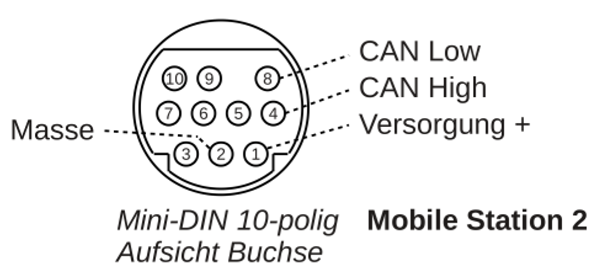
\includegraphics[width=1.00\linewidth]{../figures/mobilestation2_din10.png}
	\caption{Pinout canbus.}
	\label{fig:mobilestation2_din10}
\end{figure}

\subsection{Oscillator Settings}
Oscillator settings for the CAN peripheral need to be set up.

Open config.txt:

\begin{verbatim}
	sudo nano /boot/config.txt
\end{verbatim}

In the section for optional hardware interfaces add (if not present):

\begin{verbatim}
	dtparam=spi=on
	dtoverlay=mcp2515-can0,oscillator=16000000,interrupt=25
	dtoverlay=spi-lcs
\end{verbatim}

Use ctrl+X to stop editing, press Y and enter to save the changes.

Reboot using:

\begin{verbatim}
	sudo reboot
\end{verbatim}

To test that can0 is working properly start the connection using:

\begin{verbatim}
	sudo ip link set can0 up type can bitrate 250000
\end{verbatim}

Check the connection status:

\begin{verbatim}
	ifconfig
\end{verbatim}

In the output, can0 should be visible. Output should be similar to this (UP, RUNNING):

\begin{verbatim}
	can0: flags=193<UP,RUNNING,NOARP>  mtu 16
	unspec 00-00-00-00-00-00-00-00-00-00-00-00-00-00-00-00  txqueuelen 10  (UNSPEC)
	RX packets 0  bytes 0 (0.0 B)
	RX errors 0  dropped 0  overruns 0  frame 0
	TX packets 0  bytes 0 (0.0 B)
	TX errors 0  dropped 0 overruns 0  carrier 0  collisions 0
\end{verbatim}

Now that we know that the communication with the MCP2515 is working properly. The next step is to check if the CAN transceiver is able to listen to the CAN-bus. To do this, the CAN helper tools are needed. \\

To avoid the error: /autogen.sh: line 20: autoreconf: command not found ; execute the following commands first:

\begin{verbatim}
	sudo apt-get install autoconf
	sudo apt-get install libtool
\end{verbatim}

Install the CAN helper tools using:

\begin{verbatim}
	git clone https://github.com/linux-can/can-utils.git
	
	cd can-utils
	
	./autogen.sh
	
	./configure
	
	make
	
	sudo make install
\end{verbatim}

Now we can test the board. Connect the Gleisbox with the Mobile Station 2 and the Raspberry Pi (via the board). Power on the Gleisbox and the Mobile Station.

Monitor the CAN bus messages using the candump function:

\begin{verbatim}
	sudo ./candump can0
\end{verbatim}

Press the stop button on the mobile station a few times. Messages should appear and they should look something like this:

\begin{verbatim}
	  can0  0036936E   [5]  00 00 00 00 11
	can0  0030936E   [0]
	can0  0031931F   [8]  47 44 D8 D6 01 27 00 10
	can0  0000936E   [7]  00 00 00 00 09 00 09
	can0  0000936E   [6]  00 00 00 00 08 07
	can0  0001931F   [7]  00 00 00 00 09 00 09
	can0  0000936E   [5]  00 00 00 00 01
	can0  0001931F   [6]  00 00 00 00 08 07
	can0  0001931F   [5]  00 00 00 00 01
	can0  0000936E   [5]  00 00 00 00 00
	can0  0001931F   [5]  00 00 00 00 00
	can0  0000936E   [7]  00 00 00 00 09 00 09
	can0  0000936E   [6]  00 00 00 00 08 07
	can0  0001931F   [7]  00 00 00 00 09 00 09
	can0  0000936E   [5]  00 00 00 00 01
	can0  0001931F   [6]  00 00 00 00 08 07
	can0  0001931F   [5]  00 00 00 00 01
	can0  0030936E   [0]
	can0  0031931F   [8]  47 44 D8 D6 01 27 00 10
\end{verbatim}

When a similar output is visible, the connection with the Gleisbox and the track is established succesfully! If a retest of the CAN bus is needed; simply navigate to the folder 'can-utils' and use the command sudo ./candump can0. Exit the candump function using ctrl+C.

Now, make sure that can0 starts up automatically. Open /etc/network/interfaces:

\begin{verbatim}
	sudo nano /etc/network/interfaces
\end{verbatim}

Add the following lines:

\begin{verbatim}
	auto can0
	iface can0 can static
			bitrate 250000
\end{verbatim}

Use ctrl+X to stop editing, press Y and enter to save the changes.

\subsection{SRCPD}
The CAN bus is now fully operational. SRCPD is needed to provide the interface between the can peripheral and rocrail. To install srcpd (version 2.1.6):

\begin{verbatim}
	wget https://sourceforge.net/projects/srcpd/files/srcpd/2.1.6/srcpd-2.1.6.tar.gz
\end{verbatim}

Install srcpd (answer Yes when asked):

\begin{verbatim}
	tar -xzf srcpd-2.1.6.tar.gz
	
	cd srcpd-2.1.6/
	
	sudo apt-get install libxml2 libxml2-dev telnet
	
	./configure
	
	make
\end{verbatim}

\subsection{Rocrail Server Settings}



\begin{figure}[h!]
	\centering
	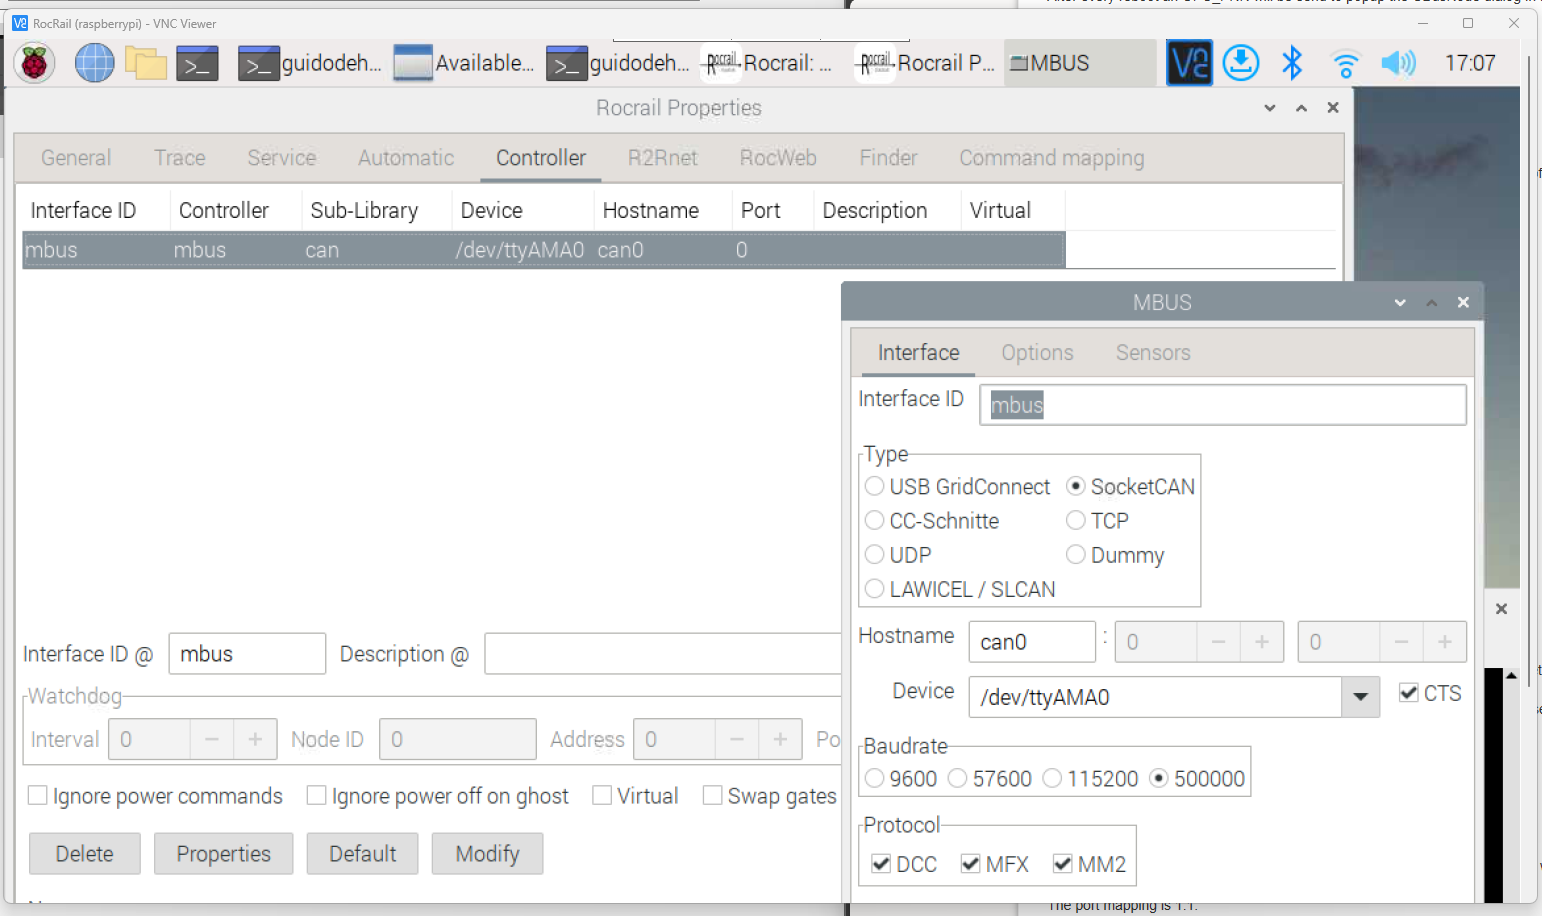
\includegraphics[width=1.00\linewidth]{../figures/rocrailServerSettings.png}
	\caption{rocrailServerSettings.}
	\label{fig:rocrailServerSettings}
\end{figure}


